\subsection{Phase-1 electronics} \label{sec:Phase1CSCelectronics}

CSC trigger and DAQ channels rely on a sequence of on- and off-chamber electronics for reading, storing, processing, and transmitting the analog signals from the strips and wires. Before explaining the Phase-2 upgrades to the CSCs, a more detailed description of the electronics prior to the upgrades---both on- and off-chamber---is necessary. 

Cathode strip signals are read by five Cathode Front-End Boards (CFEBs) mounted to each CSC (see Fig.~\ref{fig:CFEB}). A number of custom Application Specific Integrated Circuits (ASICs) fused to each CFEB are responsible for shaping, amplifying, and storing cathode strip signals and identifying hits: Buckeye ASICs amplify and shape the signals from each cathode strip before sending signals down trigger and DAQ streams; Comparator ASICs rapidly identify hits with half-strip resolution and send these downstream to an off-chamber Trigger Motherboard (TMB); and Switched Capacitor Arrays (SCAs) store strip charges in anolog form of up to six events while waiting for an L1A from the TMB. Upon reciept of an L1A the SCAs will send precision data to be digitized by Analog-to-Digital Converters (ADCs) before both data and trigger information is forwarded to an off-chamber DAQ Motherboard (DMB). Anode wire signals---``ganged'' into groups of 10-15 wires---are amplified by 42 on-chamber Anode Front-End Boards (AFEBs) and sent to an Anode Local Charged Track (ALCT) board, also on-chamber. A mezzanine on the ALCT baseboard identifies patterns among the anode hits in the six wire layers (a minimum of four layers is consistent with a muon). The two patterns with the most layer hits are sent off-chamber for processing by the TMB. A Low-Voltage Distribution Board (LVDB) on each chamber supplies power to all the electronics.

\begin{figure}[H]
    \centering
    {\includegraphics[width=1\textwidth]{Images/Phase2Upgrades/Electronics/CFEB.png}}
    \caption{One of five CFEBs used to read cathode strip signals on a CSC.}
    \label{fig:CFEB}
\end{figure}

The TMB reads the trigger primitives generated from the on-chamber electronics---Cathode Local Charged Tracks (CLCTs) from the CFEB Comparators and ALCTs from the ALCT board---and from these constructs 2D Local Charged Tracks (LCTs), requiring four layer hits, which are sent to the EMTF. The DMB builds data packets with cathode strip data from the CFEBs, Anode wire data from the ALCT (through the TMB), and trigger data from the TMB. CSC data packets from 15 DMBs corresponding to chambers in a different 20 degree sector in each station (to balance the readout load) are read by Detector Dependent Units (DDUs) with \SI{1.6}{Gb/s} links, unpacked in real-time, then merged and sent to CMS DAQ. DMBs are also responsible for controling on-chamber voltages via the LVMB and controls the CFEBs. Photographs of a TMB and DMB are shown in Fig.~\ref{fig:TMBDMB}.

\begin{figure}[H]
    \centering
    {\includegraphics[width=0.49\textwidth]{Images/Phase2Upgrades/Electronics/TMB.png}}
    {\includegraphics[width=0.49\textwidth]{Images/Phase2Upgrades/Electronics/DMB.png}}
    \caption{Left: A TMB for reading CSC trigger primitives and processing L1As. Right: A DMB for reading and transmitting precision data packets from CSCs.}
    \label{fig:TMBDMB}
\end{figure}

TMBs and DMBs are housed in ``peripheral'' VME crates, each supporting nine CSCs, secured to the edges of each ME disk (six peripheral crates per station). Each peripheral crate also houses the following: a Muon Port Card (MPC) that collects the LCTs from each of the nine TMBs in the crate and sends them to the muon track finder system; A Clock and Control Board (CCB) acting as an interface between the CSCs and the Trigger, Timing and Control (TTC) system of CMS, synchronizing the crate operations; and a VME Crate Controller (VCC) that distributes the VME commands recieved from the control room to the other boards in the peripheral crate.

\subsection{Phase-2 electronics} \label{sec:Phase2CSCelectronics}

Prior to LS1, cathode strips on each ME1/1 chamber had been divided into two groups based on pseudorapidity: ME1/1a covering $2.0 < |\eta|< 2.4$, and ME1/1b covering $1.5 < |\eta| < 2.0$. Issues observed during Run I with muon triggering in the triply-ganged ME1/1a cathode strips required unganging of the strips in all ME1/1 chambers and the a/b division removed. To accomodate the increase in channels and better cope with the trigger rate, ME1/1 chamber electronics underwent several upgrades. The five CFEBs were replaced by seven Digital CFEBs (DCFEBs) to read cathode strip signals. DCFEBs (shown in Fig.~\ref{fig:DCFEB}) continuously digitize strip signals with flash ADCs and store digitized signals in the deep buffers of a Virtex-6 Field Programmable Gate Array (FPGA). Trigger and data readout bandwidth on DCFEBs were upgraded to \SI{3.2}{Gb/s} Finisar optical links. To recieve the optical links from the DCFEBs, the off-chamber TMB/DMB were correspondingly upgraded to an OTMB/ODMB (see Figs.~\ref{fig:OTMB} and~\ref{fig:ODMB})with powerful Virtex-6 FPGAs and \SI{1.6}{Gb/s} output links. The LVDB was upgraded to an LVDB7 and the ALCT mezzanine was upgraded with a Spartan-6 FPGA (ALCT-S6, also ALCT-LX150) capable of improved algorithms for pattern finding. The CFEBs formerly on the ME1/1 chambers were adopted to construct the 72 ME4/2 chambers, which prior to LS1 had not been built due to a lack of funding.

\begin{figure}[H]
    \centering
    {\includegraphics[width=1\textwidth]{Images/Phase2Upgrades/Electronics/DCFEB.png}}
    \caption{DCFEBs used to upgrade the ME1/1 chambers in LS1 and ME234/1 chambers in LS2.}
    \label{fig:DCFEB}
\end{figure}

\begin{figure}[H]
    \centering
    {\includegraphics[width=1\textwidth]{Images/Phase2Upgrades/Electronics/OTMB.png}}
    \caption{Left: an OTMB mezzanine. Right: an OTMB baseboard. The OTMBs replaced the TMBs for ME1/1 chambers in LS1.}
    \label{fig:OTMB}
\end{figure}

\begin{figure}[H]
    \centering
    {\includegraphics[width=1\textwidth]{Images/Phase2Upgrades/Electronics/ODMB.png}}
    \caption{An ODMB used to upgrade the DMBs for ME1/1 chambers in LS1}
    \label{fig:ODMB}
\end{figure}

Radiation tests of CSC modules simulating a decade of HL-LHC data taking revealed that chambers are exceptionally robust, demonstrating adequite performance consitent with Phase-1. Even still, the higher radiation doses anticipated during Phase-2 are expected to cause certain electronic readout components on CSCs at high psuedorapidities to die. Along with mitigating radiation failure, higher PU scenarios will require a faster L1 trigger rate of \SI{750}{Hz} and latency of \SI{12.5}{\micro s}; without remedy, the analog readout of CFEBs on the inner CSC rings would lead to catstrophic event losses, as demonstrated in Fig.~\ref{fig:EventLosses}. To avoid these hazards during Phase-2, CSCs in the inner rings were refurbished with upgrades to their front-end electronics, installed during LS2, with minor upgrades to off-chamber electronics following in LS3. ME1/1 DCFEBs were replaced by more radiation-hard xDCFEBs with improved VTTx/VTRx optical recievers in place of the Finisars (see Fig.~\ref{fig:xDCFEB}). Both the new xDCFEBs and ALCT-LX100s (installed during LS1) provide PROM-less solutions for ME1/1 chambers that mitigate any failures from radiation damage. As for ME234/1 chambers, their ALCTs were upgraded to ALCT-LX150Ts (a picture of the mezzanine is in Fig.~\ref{fig:ALCT}) and their CFEBs were replaced with the disused DCFEBs from the ME1/1 chambers. The Finisar optical transeivers on the DCFEBs were replaced with VTTx links on the ME234/1 chambers to supply sufficient trigger and data readout speeds (\SI{3.2}{Gb/s}). To recieve the now optical trigger links from ME234/1 DCFEBs, TMBs were upgraded to OTMBv2s. 

\begin{figure}[H]
    \centering
    {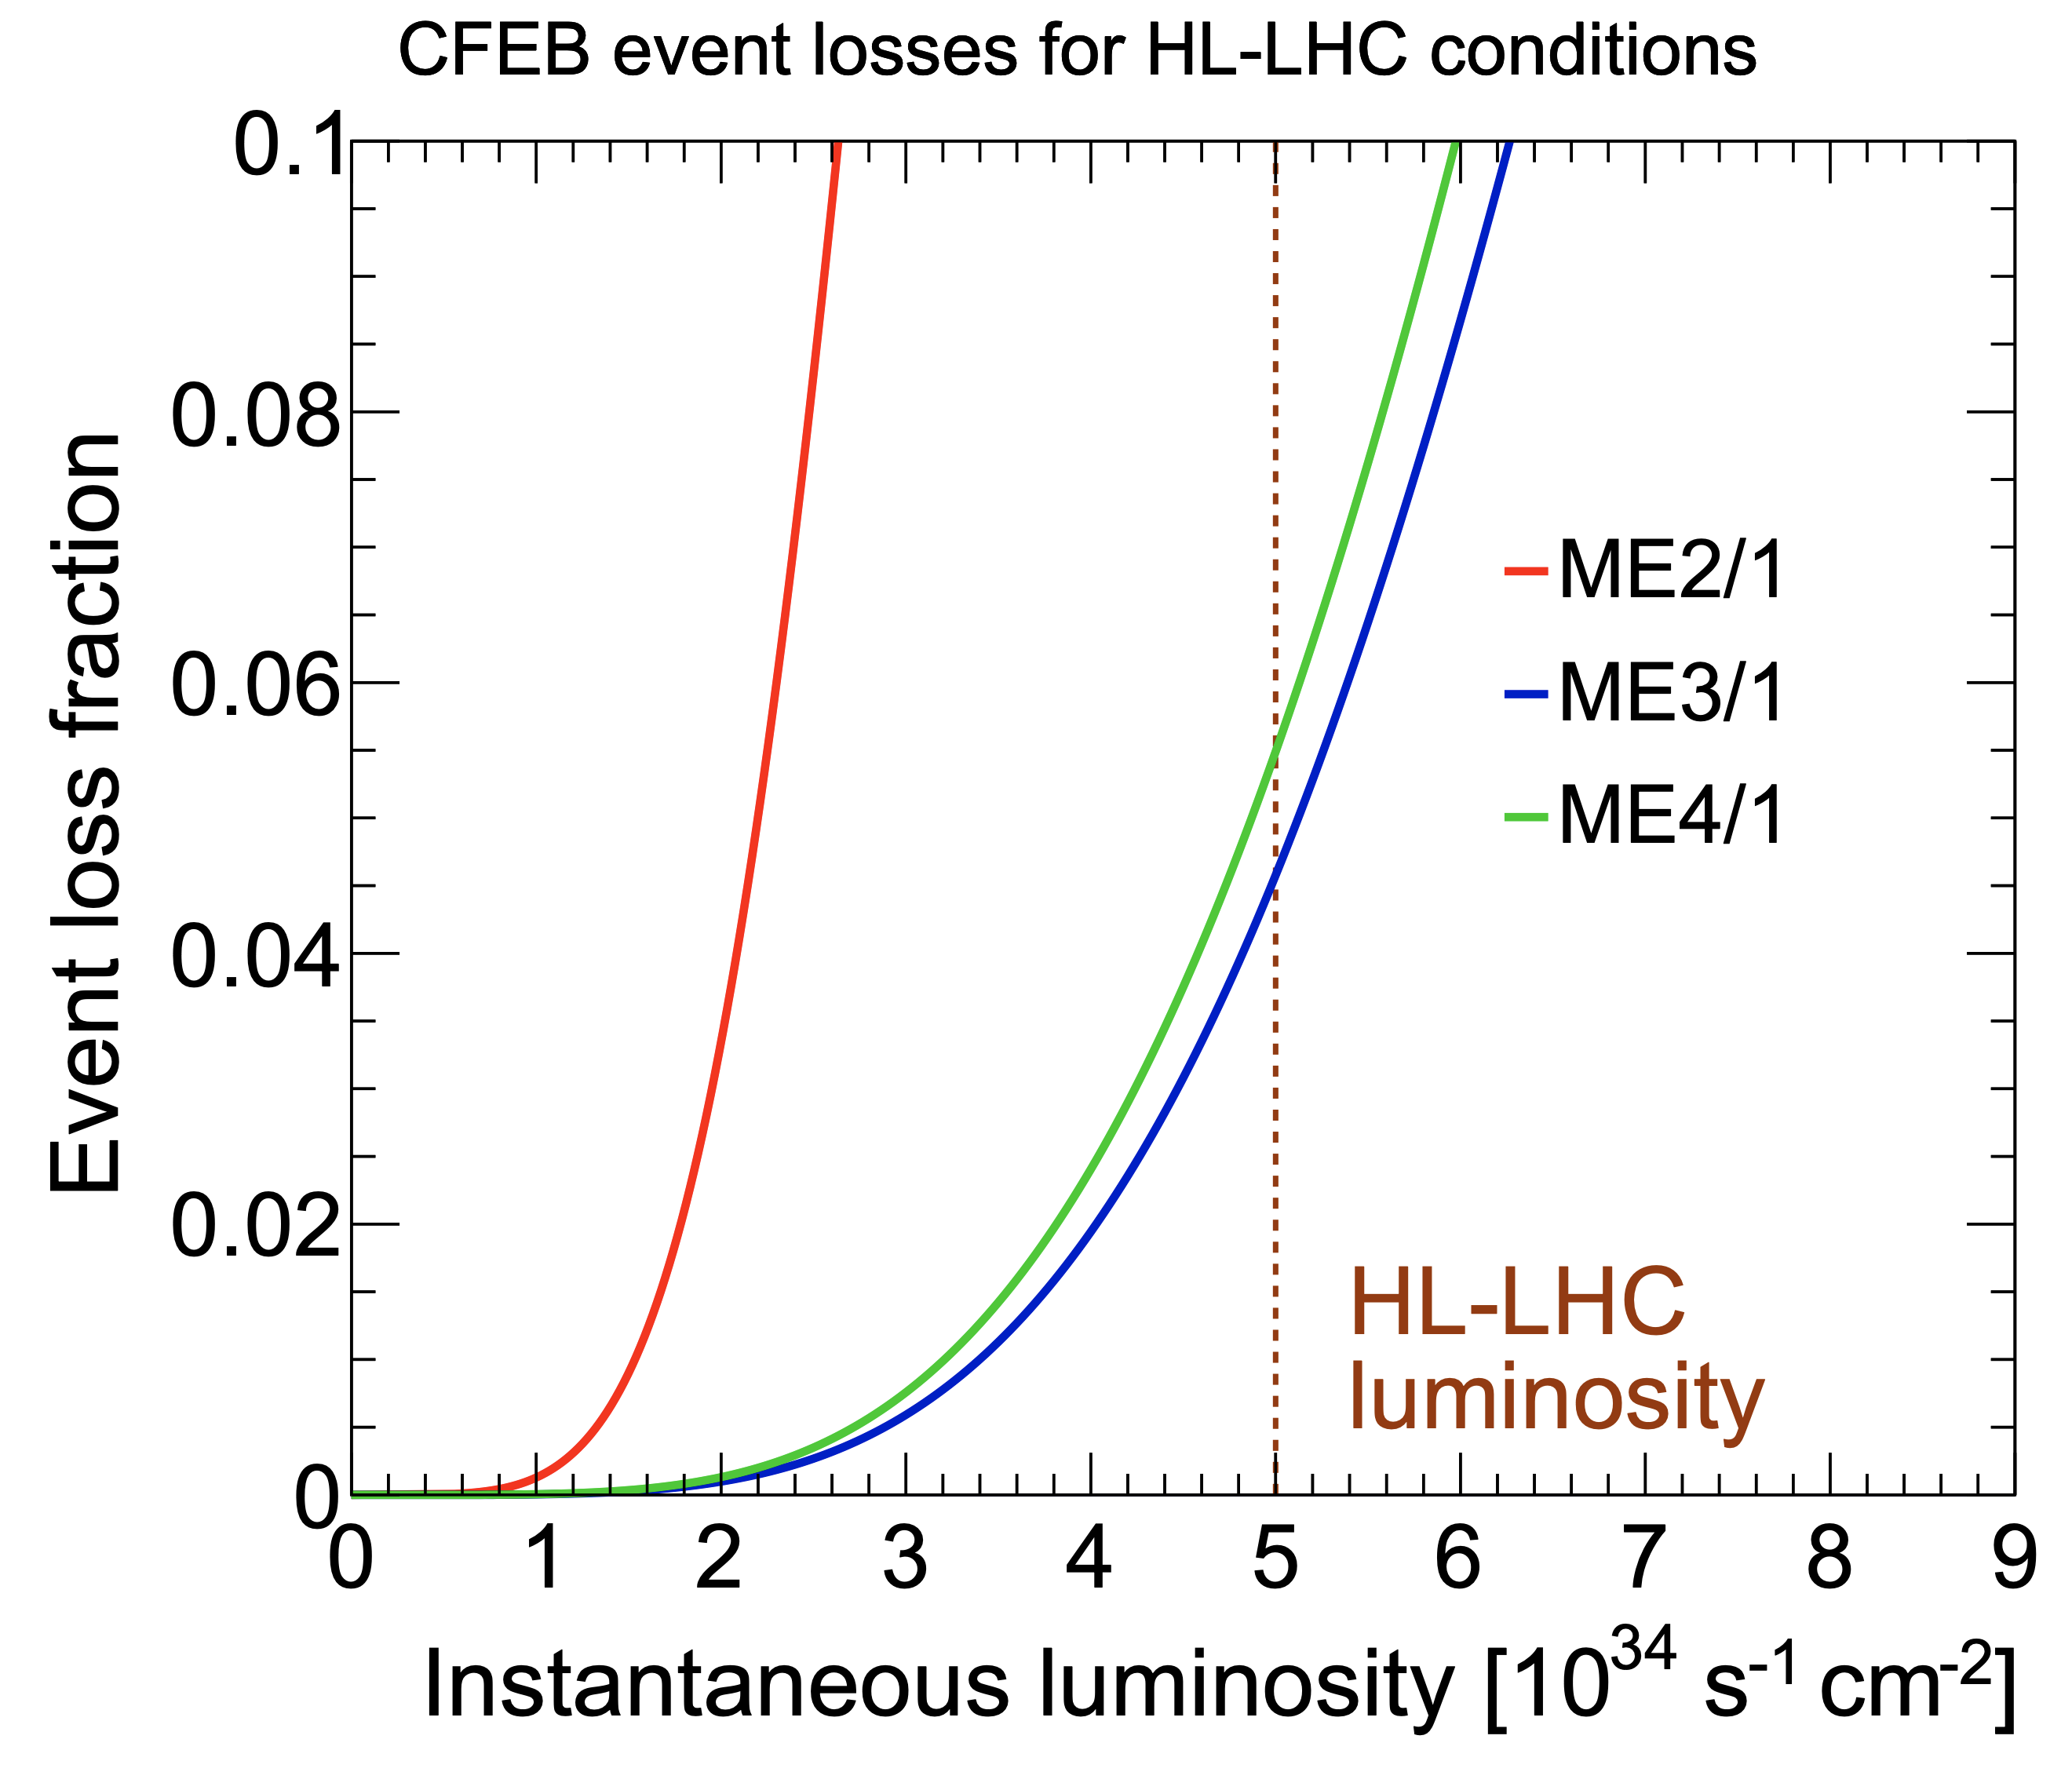
\includegraphics[width=0.49\textwidth]{Images/Phase2Upgrades/Electronics/CFEBeventlosses.png}}
    {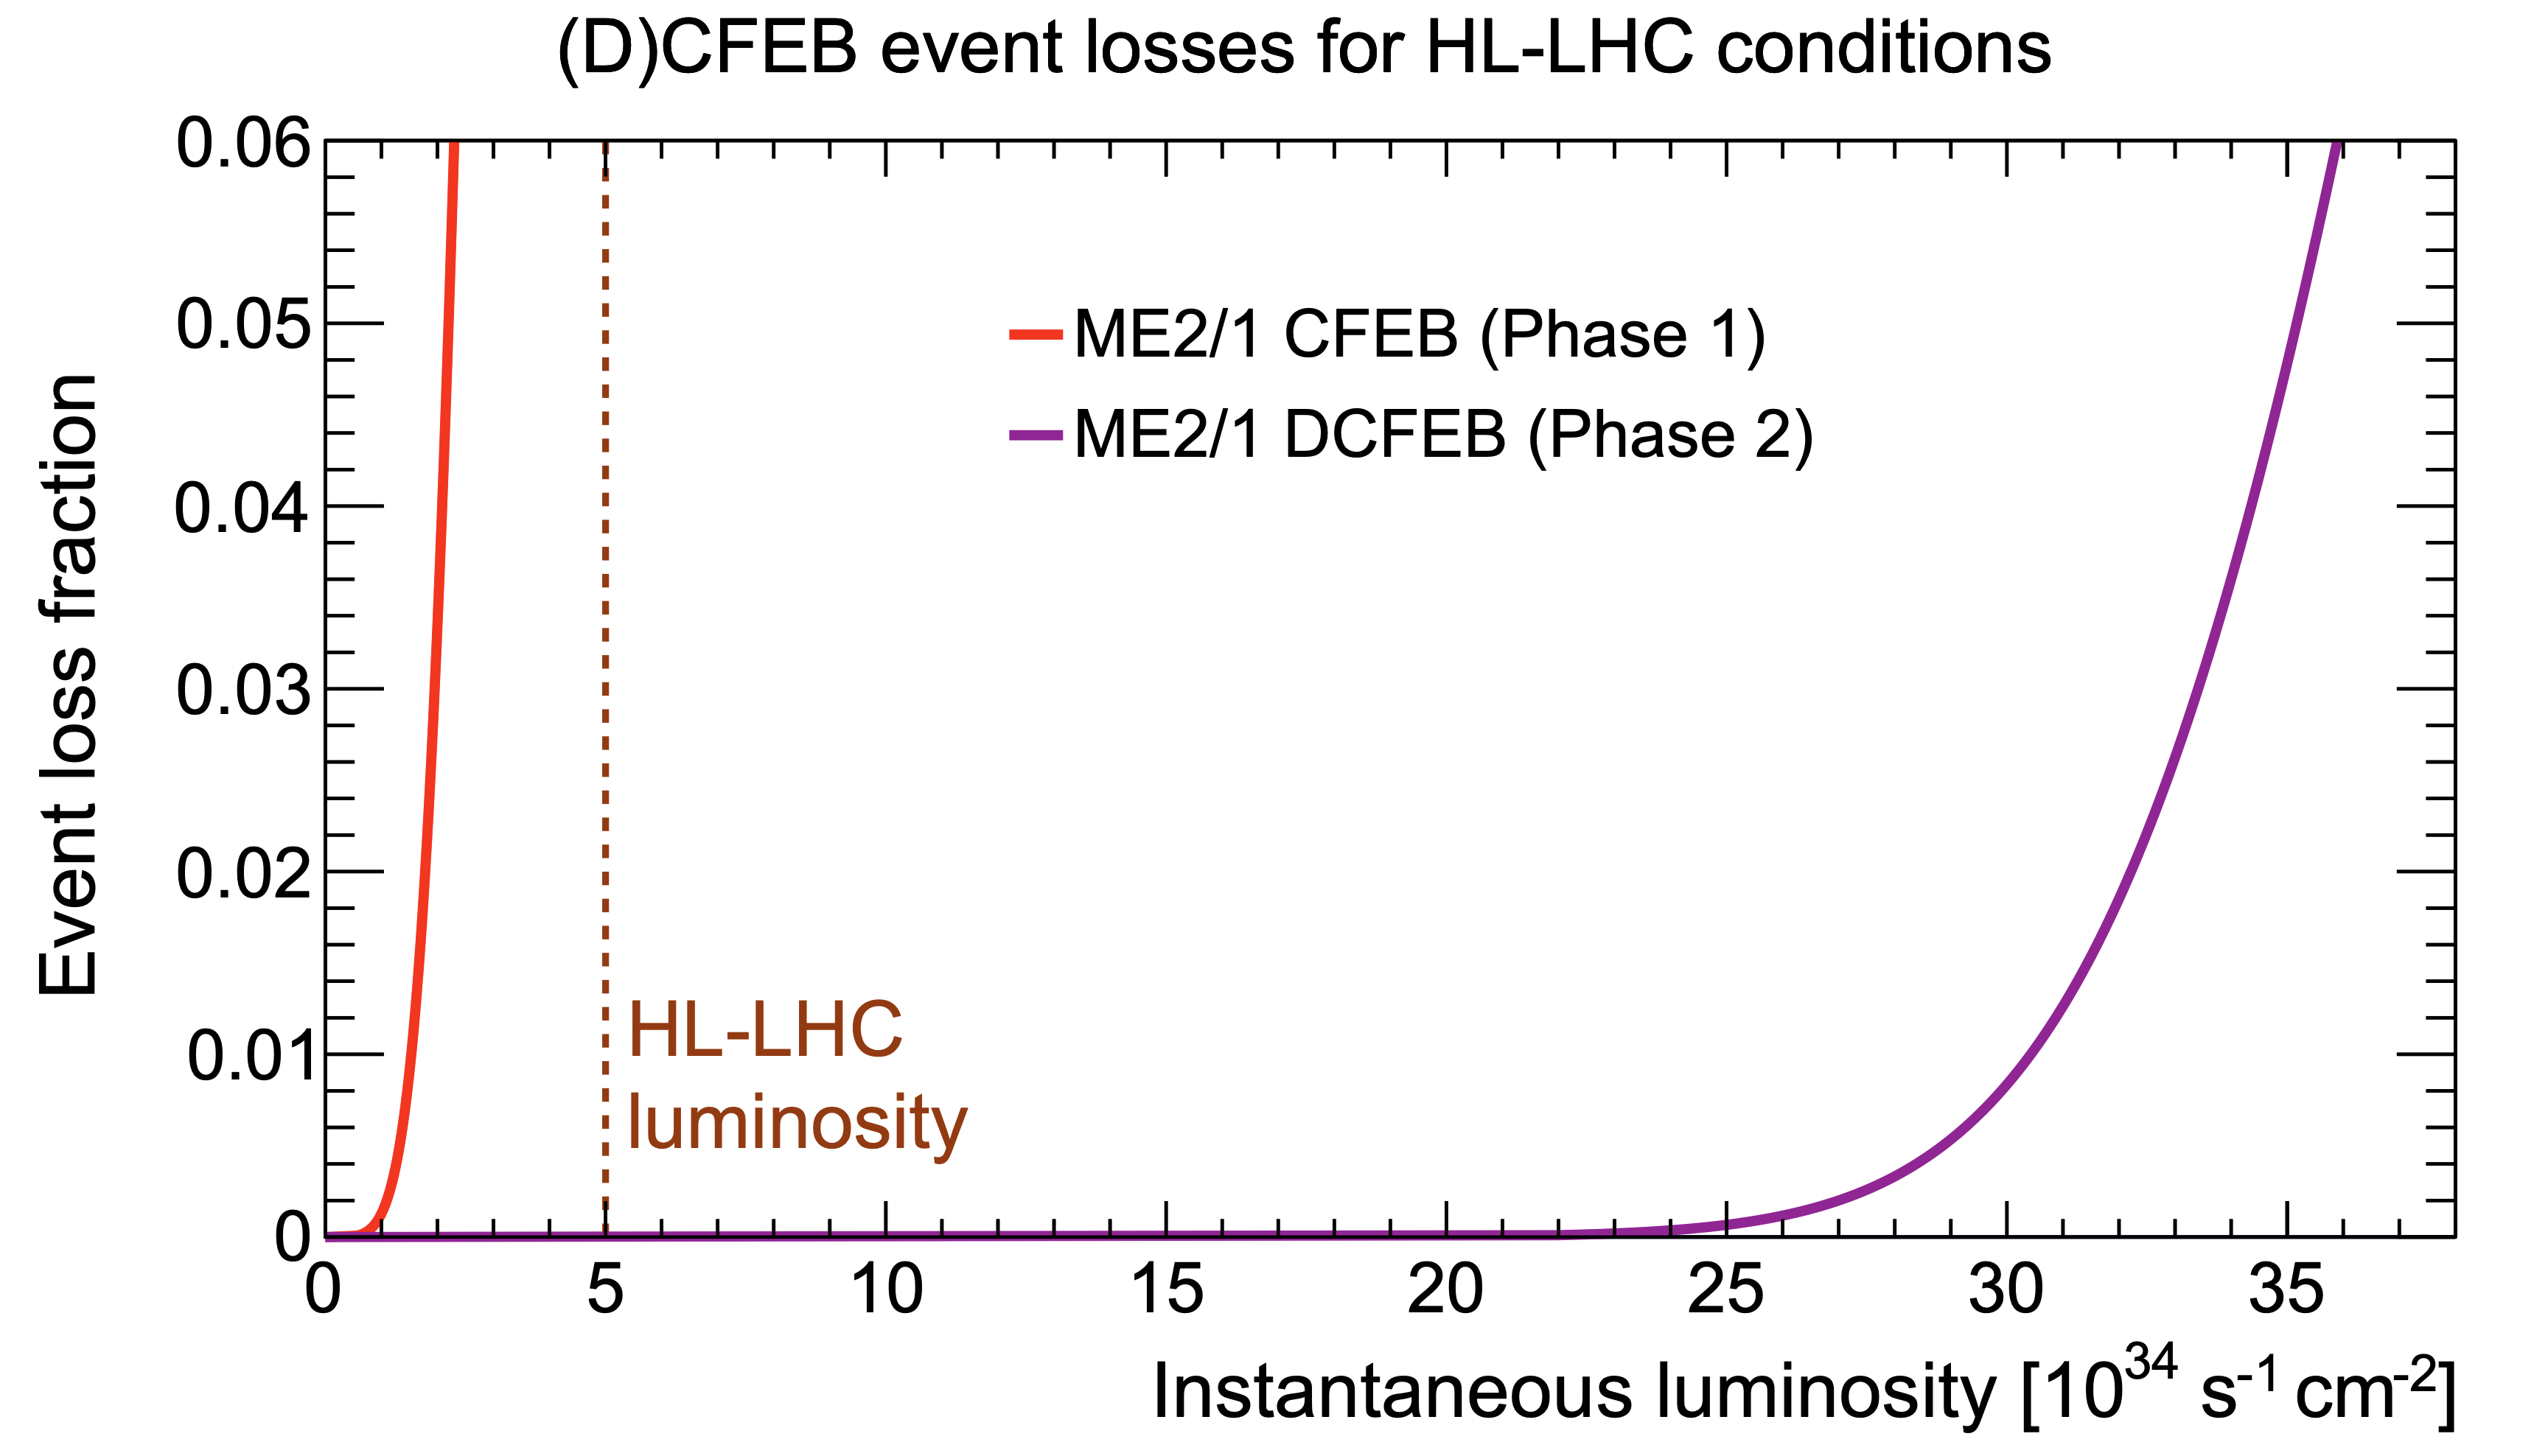
\includegraphics[width=0.49\textwidth]{Images/Phase2Upgrades/Electronics/DCFEBenetlosses.png}}
    \caption{Left: CFEB event loss fractions as a function of instantaneous luminosity on ME2/1, ME3/1, and ME4/1 chambers. Right: CFEB and DCFEB event loss fractions as a function of instantaneous luminosity on ME2/1 chambers. The plots demonstrate the need to replace the CFEBs with DCFEBs on ME234/1 chambers to avoid unacceptable data loss under HL-LHC conditions.}
    \label{fig:EventLosses}
\end{figure}

\begin{figure}[H]
    \centering
    {\includegraphics[width=1\textwidth]{Images/Phase2Upgrades/Electronics/xDCFEB.png}}
    \caption{One of seven xDCFEBs that replaced the seven DCFEBs on ME1/1 chambers in LS2.}
    \label{fig:xDCFEB}
\end{figure}

\begin{figure}[H]
    \centering
    {\includegraphics[width=1\textwidth]{Images/Phase2Upgrades/Electronics/ALCTLX150Mezz.png}}
    \caption{The ALCT-LX150 mezzanine that replaced the old ALCT mezzanines on ME1/1 chambers in LS2.}
    \label{fig:ALCT}
\end{figure}


A final set of Phase-2 upgrades will be implimented in LS3 only to off-chamber electronics. The ODMBs and DMBs of ME1/1 and ME234/1 chambers, respectively, will be replaced with ODMB7s and ODMB5s, critically increasing the output bandwidth from \SI{1.6}{Gb/s} to \SI{10}{Gb/s}. The ODMB5s will also provide optical links to the DCFEBs, replacing the legacy copper DAQ channels still in use on ME234/1 chambers throughout Run 3. An upgrade to the backend system to handle the output DAQ rates of the ODMB7 and ODMB5, featuring new FED boards for all MEx/1 chambers, will also be installed during LS3. A schematic of ME1/1 and ME234/1 CSC electronics prior to and following the Phase 2 upgrades is shown in Fig.~\ref{fig:CSCdiagram}.

\begin{figure}[H]
    \centering
    {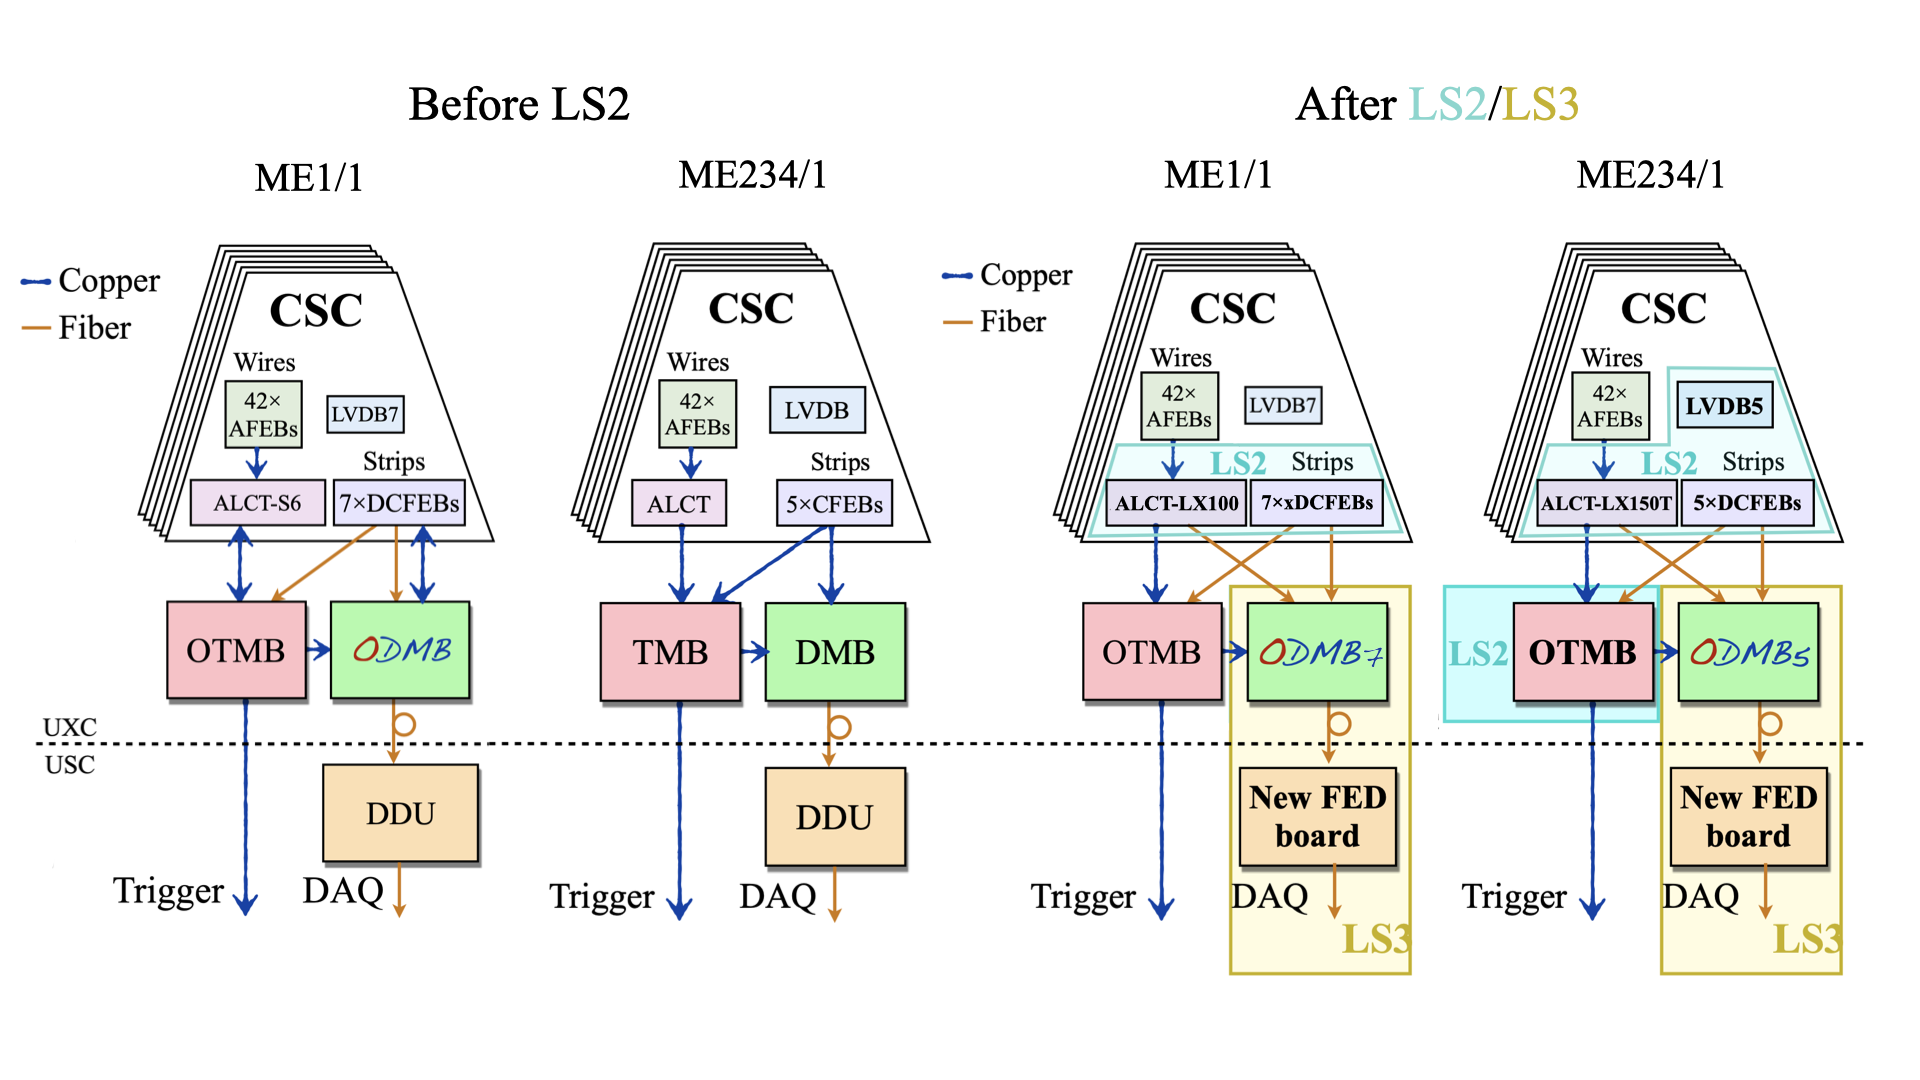
\includegraphics[width=1\textwidth]{Images/Phase2Upgrades/Electronics/CSCLS2Upgrades.png}}
    \caption{Left: Diagrams showing CSC electronics prior to LS2 on ME1/1 (far-left) and ME234/1 (second-from-left) chambers. Right: Diagrams showing CSC electronics after LS3 on ME1/1 (second-from-right) and ME234/1 (far-right) chambers. Upgrades installed during LS2 are highlighted in blue, while upgrades planned for LS3 are highlited in gold.}
    \label{fig:CSCdiagram}
\end{figure}